
\chapter{Implementation}
\label{sec:implementation}
\noindent

\noindent In this chapter, we provide a detailed implementation of our proposed methodology. We start with presenting the platform we incorporated to shape and design our model. Then we demonstrate our network's architecture in detail. Finally, we attempt to give insight into the datasets we used to train and test our model. 

\section{Caffe deep learning platform}

Caffe is a clean and modifiable framework for state-of-the-art deep learning algorithms and a collection of reference models. The framework is a BSD-licensed C++ library with Python and MATLAB bindings for training and deploying general-purpose convolutional neural networks and other deep models efficiently on commodity architectures. It powers on-going research projects and large-scale industrial applications in vision, speech and multimedia by CUDA GPU computation (CUDA is a parallel computing platform and application programming interface (API) model created by NVIDIA\cite{cuda}), processing over 40 million images a day on a single K40 or Titan GPU\cite{jia2014caffe}. 
The main components of Caffe architecture are listed and succinctly explained in below:
\begin{enumerate}
\item \textbf{Data storage:} Caffe stores and communicates data in 4-dimensional arrays called \textit{blobs}. Blobs provide a unified memory interface, holding batches of data, parameters, or parameter updates. Blobs conceal the computational overhead by synchronizing from the CPU host to the GPU device as needed. Caffe supports some data sources such as LevelDB or LMDB, HDF5, MemoryData, ImageData, etc. However, large-scale data is stored in LevelDB data bases since it reads the data directly from memory\cite{caffe}. 
\item \textbf{Layers:} A caffe layer takes blobs as input and yields one or more as output. In a network, each layer plays two important roles: a forward pass that takes the inputs and produces the outputs, and a backward pass that takes the gradient with respect to the output, and computes the gradients with respect to the parameters and to the inputs, which are in turn back-propagated to earlier layers \cite{jia2014caffe}.

\indent Caffe affords a exhaustive set of layers including: convolution, pooling, fully connected, nonlinearities like rectified
linear and logistic, local response normalization, element-wise operations, and losses like softmax and hinge \cite{jia2014caffe}.  
\item \textbf{Networks and run mode:} Caffe ensures the correctness of the forward and backward passes for any directed acyclic graph of layers. A typical network begins with a data layer laying at the bottom going up to the loss layer that computes tasks' objectives. The network is run on CPU or GPU independent of the model definition. 
\item \textbf{Training a network:} Training phase in Caffe is done by classical stochastic gradient descent algorithm. When training, images and labels pass through different layers to be fed to the final prediction into a classification layer that produces the loss and gradients which train the whole network. Figure~\ref{fig:caffe} illustrates a typical example of a Caffe network. 

\indent Finetuning, the adaptation of an existing model to new architectures or data, is a standard method in Caffe. Caffe  finetunes the old model weights for the new task and initializes new weights as needed. This capability is essential for tasks such as knowledge transfer \cite{donahue2013decaf}, object detection \cite{girshick2014rich}, and object retrieval \cite{guadarrama2014open} \cite{jia2014caffe}.  
\end{enumerate}

\begin{figure}[H]
	\centering
	{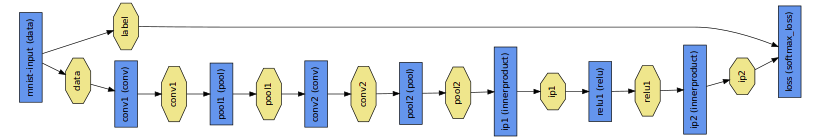
\includegraphics[width=1\textwidth]{images/caffe}}
	\caption{An MNIST digit classification example of a Caffe network, where blue boxes represent layers and yellow octagons represent data blobs produced by or fed into the layers\cite{jia2014caffe}.}
	\label{fig:caffe}
\end{figure}

We decided to use Caffe because, it addresses computation efficiency problems (as likely the fastest available implementation of deep learning frameworks), adheres to software engineering best practices, providing unit tests for correctness and experimental rigor and speed for deployment. It is also well-suited for research use,due to the careful modularity of the code, and the clean separation of network definition (usually the novel part of deep learning research) from actual implementation\cite{jia2014caffe}. Moreover, providing Python wrapper which exposes the solver module for easy prototyping of new training procedures. 

\section{The architecture}

In learning features or object representations for vision tasks and by the use of neural networks, the depth of network plays an important role. The deeper the model, the better it learns. However, issues like overfitting and underfitting should not be left neglected.   
Having Caffe platform introduced, we propose the designed network for two experiments we did regarding learning to count problems. Therefore, in this section, networks' settings and architectures for even digit recognition and crowd counting problems will be described separately. 

\subsection{Even digit recognition}

For learning to count even digits problem, since we used MNIST dataset to generate our dataset, we decided to start with an architecture similar to the classic MNIST hand-written digit recognition problem\cite{lecun1995comparison}. From there, we modified the architecture to optimize the performance of the network.

\indent In our network, the data layer fetches the images and labels from the disk, passes it through, the first convolutional layer with 20 filters, each of size 15*15 followed by a ReLU non-linearity and LRN normalization layer. Then the output is pooled by the size of 2*2. This process repeats again but this time with the second convolutional layer having 50 filters of size 3*3. In all convolution and pooling layers, the \textit{stride} = 1 and \textit{padding} = 1 are considered. Afterwards,

\begin{wrapfigure}[45]{r}{0.58\textwidth}
  \centering
   {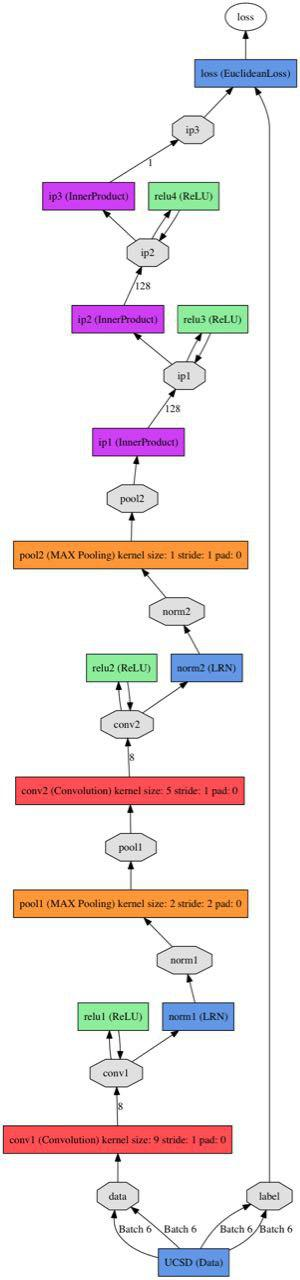
\includegraphics[width=0.33\textwidth]{images/model}}
  %\end{center}
	\caption{Proposed network architecture for Even digits recognition task}
	\label{fig:l2cNet}
\end{wrapfigure}

\noindent the output of the second pooling layer is fed to two fully connected (inner product) layers with respectively 64 and 1 number of outputs (since the problem is approached as a regression task). Both fully connected layers are followed by ReLU non-linearities. Figure~\ref{fig:l2cNet} shows a schematic of the architecture. In addition, parameters of the network are set as below:
\begin{itemize}
\item \textbf{Learning rate:} The basic learning rate is 0.0001. However, for our experiment we chose \textit{multi-step} learning policy in which, after each \textit{stepsize}=40000 iterations, the learning rate drops by the rate of $\gamma = 0.1$. This initialization is based on rules of thumbs used in \cite{krizhevsky2012imagenet}.
\item \textbf{Momentum:} We use momentum $\mu = 0.9$. This selection also is based one rules of thumbs. Because, momentum setting $\mu$ effectively multiplies the size of our updates by a factor of $\frac{1}{1-\mu}$. Hence, changes in momentum and learning rate ought to be accompanied with an inverse correlation. When momentum $\mu = 0.9$, we have an effective update size of 10 since we also drop the learning rate by the factor of $\gamma= 0.1$.
\item \textbf{Weight decay:} Weight decay as a penalty term to the error function, has a constant value of 0.0005. This decay constant is multiplied to the sum of squared weights.
\end{itemize}

\noindent We should also mention that at the top layer of the network, we used \textit{Euclidean Loss }layer to compute  the euclidean distance between the predictions and ground truth. 

\begin{wrapfigure}[44]{r}{0.58\textwidth}
  \centering
   {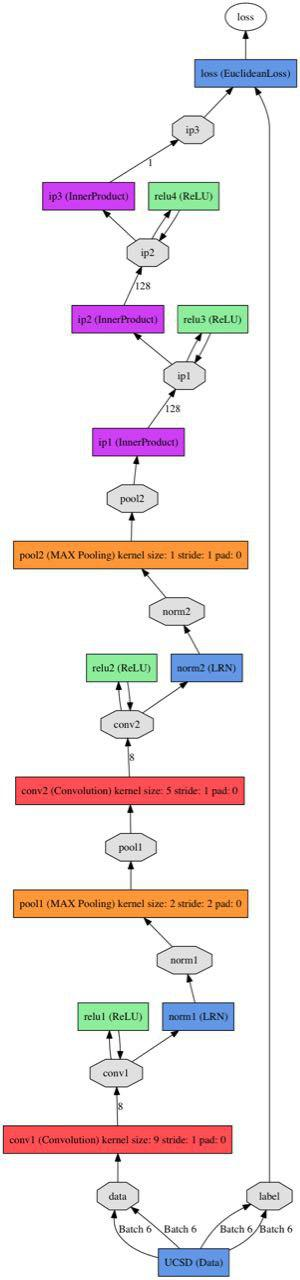
\includegraphics[width=0.31\textwidth]{images/model}}
  %\end{center}
	\caption{Proposed network architecture for Even digits recognition task}
	\label{fig:l2cNet}
\end{wrapfigure}
%\newpage
\subsection{Crowd counting}

In the case of counting pedestrians task, we applied the same settings to a different architecture. This time, due to more complexity of images, we considered a deeper network. Here the data blobs pass through 4 convolutional layers. First convolutional layer has 4 filters, each with 5*5 kernel and the other 3 layers have again 4 filters but each of size 3*3. Similar to the previous model, each convolutional layer is followed by ReLU non-linearity layer and LRN normalization layer. Also the stride and padding values for all the convolutional layers are respectively equal to 1 and 0. 

\indent In order to not lose information, we used merely two pooling layers for the first two convolutional layers. Each pooling layer has a kernel size of 2*2 with stride = 1 and padding = 0. 

There are three fully connected layers to regress the number of pedestrians in images. The first two fully connected layers have 16 outputs each and are connected to ReLU non-linearity layers. The last layer however, with solely one output, passes the models' prediction of the number of pedestrians to the Euclidean loss layer to calculate the sum of squares of differences of its two inputs, the true labels and predictions.  

To the best of our knowledge and experience, the designed architectures outperform the other architectures while fasten the training phase. However, apart from the basic knowledge about network architectures, hyper-parameters initialization and some rules of thumbs of successful experiences in similar works, the rest of design has been done intuitively.

\section{The datasets}

Now, we delve into the data processing part of this work by introducing three different datasets we generated or chose for our empirical experiments. To that end, we provide a detailed explanation of the approaches and methods used to generate and improve each dataset.

\subsection{Even-odd digits dataset}

For the first analysis,we used original MNIST dataset \cite{lecun1998mnist} to create our set of images. MNIST dataset contains a training set of 60,000 examples and a test set of 10,000 examples. Each image has a size of 28*28 with one random hand-written digit centered in the image. 
An example of original MNIST is depicted in the below figure.

\begin{figure}[H]
	\centering
	{
\includegraphics[width=0.25\textwidth]{images/mnist}}
		\caption{An example of original MNIST data with hand-written digit number 4 in the image. }
	\label{fig:mnist}
\end{figure}

Our Even-odd handwritten dataset contains images of size 100*100. Each image is filled with 0 up to 15 randomly selected digits from MNIST dataset. Digits are resized to 18*18 pixels and randomly put in the image. The images are created with controlled overlapping by ensuring that two different numbers are 18 pixels away from each other, i.e. the distance between two digits centers is larger than 18 pixels. For the training process, images are labeled with the number of even digits present in each image. Figure~\ref{fig:l2cmnist} illustrates some examples of even-odd digits dataset with different number of even digits in images. 

\begin{figure}[H]
	\centering
	{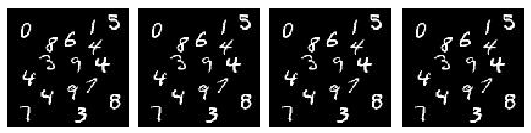
\includegraphics[width=0.9\textwidth]{images/l2cmnist}}
		\caption{An example of even-odd digits images. Form left to right, images contain 0, 5, 10 and 15 even digits.}
	\label{fig:l2cmnist}
\end{figure}

\indent This dataset has in total 1 million images, 800,000 images for training set and 200,000 as the test. Also, the dataset is uniformly generated, meaning that for instance, the number of images containing 0 even digits are equal to the number of images containing 15 even digits.  

\subsection{Synthetic pedestrians dataset}

Learning features using deep architectures require a large amount of data. More importantly, for a fully supervised learning, this data should be annotated. Lack of data or its' High annotation cost prohibit the usage of deep learning methods for many problems including Crowd counting. 

\indent However, in order to soften this cost, in our research, we decided to synthetically generate a data set of pedestrians in a walkway. To do that, we used UCSD unlabeled dataset of pedestrians used in \cite{chan2009analysis, mahadevan2010anomaly, li2014anomaly}. UCSD Anomaly detection dataset contains clips of groups of people walking towards and away from the camera, and some amount of perspective distortion. Contains 34 training video samples and 36 testing video samples. Each video has 200 frames.

\indent In our study, we used the 36 testing video samples to generate the synthetic pedestrians dataset. To pore over the generation of our dataset, we divide this process into data generation and data improvement.

  
\subsubsection{Data generation}

In our dataset, we constrained each image by having up to 30 pedestrians in the walkway. The process of generating the data includes the following steps:
\begin{enumerate}

\item \textbf{Background extraction:} Firstly, we simply subtract the background from each video frame. We extract two types of backgrounds, the median of all the backgrounds in each video(in total, 36 different backgrounds), and the median of all median backgrounds.

\item \textbf{Pedestrian extraction:}

\item \textbf{Pedestrian's impersonator creation:}

\item \textbf{Background generation:}

\end{enumerate}

\subsubsection{Data improvement}



\subsection{UCSD crowd counting dataset}